\chapter{Discussion}

\textbf{3 + 5 (Modellering)}

In chapter \ref{ch:likelihood_theory} we concluded that the MLE is efficient and therefore the unbiased estimator that minimizes variance.
There exist regularization, which introduce bias into the regression solution and thereby reduce variance compared to OLS (which in our case is equivalent to the MLE). 
This is, depending on the method, done by forcing the sum of the absolute value of the regression coefficients to be less than a fixed value.
This then forces certain coefficients to be set to zero, effectively choosing a simpler model that does not include those coefficients.
This both makes the model more interpretative and reduces over-fitting/variance.
This simpler model in turn risks under-fitting and thereby more bias.

% It is possible that we may be able to trade some bias for lower variance.
% high bias = under-fitting.
% high variance = over-fitting. 
% irreducible error: noise inherent in the observations.
% Regularization: Reduce variance for OLS, while introducing bias.
% LASSO: 

\textbf{4 + 6 (Variance/Bias Trade-off)}


\textbf{2 (Sammenligning af metoder (svært))}

\textbf{1 (Metoder i CV (k = n)}
As earlier stated in ection \ref{sec:CV}<is another common choice for k fold cross-validation k = n
\begin{figure}[H]
        \centering
      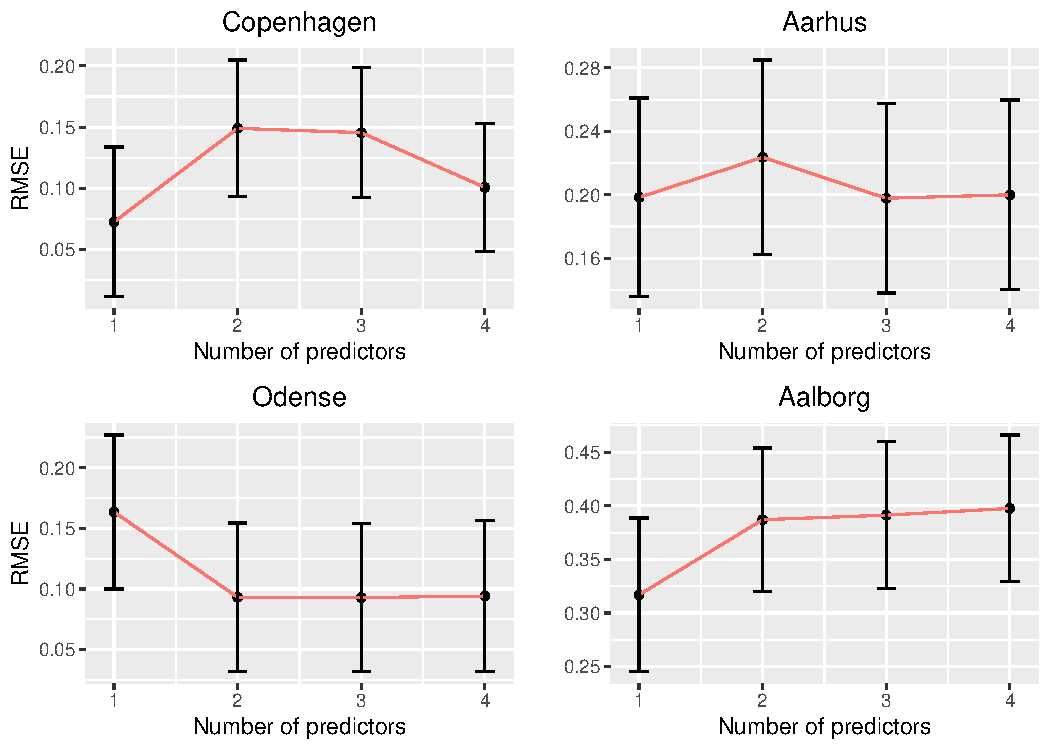
\includegraphics[width = 0.7 \textwidth]{figures/Nanna/k=n.pdf}
      \caption{Result from $k = n$ fold cross-validation.}
      \label{fig:error_cont}
\end{figure}